\chapter{\molsturm: Flexible and modular quantum-chemistry package}
\chaptermark{\molsturm quantum-chemistry package}
\label{ch:Molsturm}
\chapquote{[C has] the power of assembly language and the convenience of \ldots assembly language.}{Dennis Ritchie~(1941--2011)} \\
\chapquote{Keep it simple, make it general, and make it intelligible.}{Doug McIlroy~(1932--present)}

\todoil{Statistics: Lines of code}
\todoil{Maybe describe idea behind code structure}
Historically the \fortran library ARPACK~\cite{Lehoucq1998}

% points in need for modular
Pickup on idea of basis-type independent \SCF
Lazy matrix formalism helps
\contraction-based \SCF hard to achieve in non-flexible standard
Q-Chem programs

\lazyten is the linear algebra interface of \molsturm.
It not only implements the lazy matrix datastructures,
which define the common interface of \gint and \gscf,
but further contains code to make standard external
iterative or direct solver implementations available
from a lazy matrices-based setting.

Similarly the eigensolvers can be accessed from \gscf via a common interface,
which abstracts the precise algorithm and allows \lazyten to make an automatic
choice by looking at the precise structure of the Fock matrix at hand.

\todoil{Lazyten common interface for different numerical structure
depending on basis function type}
\todoil{Automatic choice by introspection or alternatively
	supply keywords to influence solver algortihms directly}

This chapter follows closely the ideas we presented in \cite{molsturmDesign}.

\section{The need for modular quantum chemistry software}
\todo[inline,caption={}]{
	\begin{itemize}
		\item pyscf \cite{Sun2017}
	\end{itemize}
}

\subsection{The need for a flexible quantum chemistry software platform}

% TODO Ideas of Tobias Setzer:
% Typical programs are ASCII-in -> ASCII-out
% An idea going in a similar direction is for example TURBOMOLE
%   -> apparently they have very modular modules, where the state of a compuation
%      is incoded in the file on a harddrive
%   -> issue is getting out of the TURBOMOLE ecosystem
% Actual analysis, which is not part of the program package is compartively difficult.
% Especially the transfer of data from one package to another is extremely tough.
%
% Molsturm:
%     fully dynamic, real-time analysis
%     future of molsturm: overcome software package boundaries
%     Journals: JCTC, JCP  (siehe turbomole jungs)
%
% Overall: Focus more on the advantages of the package architecture


% TODO copy -> build into this section
Most existing quantum-chemistry packages
are built around a 
particular basis function type: either Gaussians,
Slaters, or numerical orbitals. This is hard-coded 
deeply in the programs, which are usually enormous
projects written in  highly optimized \cpp or \fortran.
This makes experimentation with different and more physically
appropriate basis functions exceedingly difficult:
even when all electronic integrals have been worked out,
adapting an existing quantum chemistry code to use
them is a daunting project.
% end copy



% TODO Flowify
\todoil{Check and enhance the story by looking at more references}
Starting from the exponential form of the analytical solutions of the
Schrödinger equation for hydrogen,
\citeauthor{Slater1930} started introducing exponentially decaying basis functions
in order to compute atomic properties,~\cite{Slater1930}
the nowadays well-known Slater-type orbitals~(STOs).

Applying the STOs to molecules turned out to be much more
challenging due to the demanding structure of the electron repulsion integrals~(ERIs)
for such types of basis functions.
\todoil{I cannot download that paper so im not too sure what is in it}
In \citeyear{Boys1950} \citeauthor{Boys1950} realised that employing
atom-centered Gaussian type basis functions~(GTOs) leads to integrals
which are much easier to evaluate numerically.

Since they do, however, not describe the physical reality as closely as STOs
\todoil{Check whether the pople paper goes into this}
much larger GTO basis sets are needed to get similar accuracies than STOs.

John Pople
\todoil{Paper: Hehre, W. J.; R. F. Stewart; J. A. Pople (1969). "Self-Consistent Molecular-Orbital Methods. I. Use of Gaussian Expansions of Slater-Type Atomic Orbitals". Journal of Chemical Physics. 51 (6): 2657–2664. Bibcode:1969JChPh..51.2657H. doi:10.1063/1.1672392.}
later realised that one could combine the best of both worlds if one used
basis sets of contracted GTOs.
This set off a vivid development of quantum chemical theory and software packages,
where a lot of work has gone into efficient algorithms
improving the computational
scaling as well as the overall runtime of calculations based on GTOs.
scaling as well as the overall runtime of calculations.
\todoil{Examples for program packages ??}
% end flowify

Almost all major quantum chemistry programs,
\todoil{Cite a few}
which are actively developed nowadays focus on Gaussian-type
basis functions or Gaussian-type orbitals~(GTOs) as they are usually called.
Compared to the Slater-type orbitals~(STOs)
they certainly have a couple of well-known advantages.
Most importantly the structure of the electron repulsion integrals~(ERIs)
is much less demanding and hence makes it feasible to model much larger systems.

The downside of GTOs is of course that they do not describe the physical
reality that well and as a result fail to capture all of the properties
of an electronic structure in a truely black-box fashion.
For example the computation of proper electron affinities or the description
of Rydberg-like excited states requires incorporating diffuse functions
with small Gaussian exponents into the GTO basis set.

As such it is not surprising that other types of basis sets have been attempted as well.
Next to plane-waves or projector-augmented wave methods,
which are commonly employed in the density-functional theory~(DFT)
calculations of metal surfaces,
recently a couple of projects have also investigated the use
of so-called numerical basis functions.
Examples would be the use of wavelets and the finite-element medhod.
\todoil{Cite madness and Dage Sundholm}
\todoil{The Jensen review paper has a couple of nice citations there}

% structure is vastly different
% need flexible framework to try them
% how do they compare -> need fair comparison

\begin{figure}
	\centering
	\missingfigure{The fock matrices are not yet in the diss framework}
	%\includegraphics[scale=0.5]{img/matrices/fe.pdf}
	%\includegraphics[scale=0.5]{img/matrices/sturmian.pdf}
	%\includegraphics[scale=0.5]{img/matrices/gaussian.pdf}
	% Different numerical properties of basis functions
	% (show for sturmian vs. GTOs vs. FE)
	\caption{The different structure of the Fock matrix when FEs,
		Sturmians and GTOs are used.
		All matrices are shown early in the SCF process with a Pulay error norm
		larger than 0.1.
		The matrix structures generally improve as the SCF proceeds and contain more zeros.
		%
		Sturmian and Gaussian are almost diagonal dominant,
		even almost strictly diagonal dominant,
		FE matrix is far from it (About half the rows do not satisfy the condition).
		%
		Only the alpha-alpha part of the fock matrix is shown in each case
		and we perform an RHF calculation of the Berylium atom in a small basis
		for each set of basis functions.
		%
		The Sturmian basis is given in lmn order.
		% TODO maybe use mln order ?
	}
	\label{fig:FockStructure}
\end{figure}

The structure which is required in a program package in order to perform even a simple
self-consistent field~(SCF) calculation
based on GTOs and on numerical basis functions differs quite a lot.
As can be seen in \fig~\ref{fig:FockStructure} the structure of the Fock matrix
varies rather dramatically depending on the type of basis function,
which is used.
Most importantly the matrix size and matrix sparsity properties
changes a lot between numerical approaches like
Wavelets or Finite Elements and classical atom-centered AO approaches like GTOs.
As a result none of the widely used program packages
focus on exactly one type of basis function and are highly specific for exactly this type.

Since the structure of the numerical problems to be solved differ
implementing further basis function types into existing packages
is often challenging.
Moreover unlike the well-understood Gaussians in novel basis function types
the kind of solver algorthims to use is less clear and one often needs to be able to experiment.
\todoil{
all separate packages 
see wikipedia page
\url{https://en.wikipedia.org/wiki/List_of_quantum_chemistry_and_solid-state_physics_software}
}
Furthermore we only know of very few programs which have more than experimental
support in more than one type of basis function.
\todoil{I do not want to make this statement to harsh to piss anyone off,
	but the point is that those packages, which do exist are either not widespread
	or lack features in some of the basis functions
	or are hard to obtain (i.e. closed-source, even wikipedia knows no website)
	or I have literally not heard of them anywhere}

\todoil{I feel some more details introducing SCF in general is also appropriate here}

In previous work we have investigated the use of so-called generalised Sturmians as basis functions
in electronic structure theory.
%
\todoil{I think this is already done in one of the previous chapters in the diss}
Generalised Sturmians $\Phi_\nu(\rpack)$ are the solutions to $N$-body Schrödinger-like equation
\begin{equation}
	\left( -\frac12 \sum_{j=1}^N \Delta_j + \beta_\nu V_0(\rpack) - E \right) \Phi_\nu(\rpack) = 0
	\label{eqn:GenSturm}
\end{equation}
where $V_0(\rpack)$ is
a zero-th order potential.

In case of atoms a good choice is the nuclear attraction:
The electrostatic electron-nucleus interaction
\[
	V_0(\rpack) = - \sum_{j=1}^N \frac{Z}{r_j}.
\]
\todoil{Is many nuclei also possible here?}
Note that the electron-nucleus interaction is scaled by the factor $\beta_\nu$ in \eqref{eqn:GenSturm}
such that the solutions $\Phi_\nu(\rpack)$ all become isoenergetic.
This makes Sturmians reproduce the correct long-range decay behaviour of the electron density
as well as properly represent the nuclear cusp at the core.
As such the functional form of generalised Sturmians is very much related to STOs.
Unlike STOs the two-electron integrals can, however, be reformulated in a particular way
to make computing them less demanding.
This requires, however, that the mathematical properties of the Sturmians
can be fully exploited during the computation,
which in turn requires the Fock matrix to be arranged in a specific way.
Moreover it is advantageous to not build the coulomb and exchange matrix in memory at all,
but much rather only use these matrices in the form of matrix-vector products,
since this overall saves an order of magnitude in the computational scaling.
%
\todoil{How much shall we go into detail here to make this clear?}
% Not at all, do it in the lazyten section.
%
This rather unusual demand turned out to make it very difficult to implement Sturmians
as a basis function type into existing packages alongside STOs and GTOs.

% TODO do this do this
\todoil{Go a bit more into why we only do SCF (Explain: Post-HF available, we only need MO basis, structure of AOs not important)}
% TODO do this do this
In \molsturm we have achieved to write an Hartree-Fock SCF code,
which allows us to use both GTOs and Sturmians side by side by the means
of so-called lazy matrices (see section \ref{sec:lazymat}).
We achieve true generality in the type of basis function to be used
up to the point where most of our code is entirely
independent of the basis function types.
Enwrapping \molsturm into a \python layer allowed us to easily re-use existing
software modules (\adcman and \pyscf) in order to go beyond Hartree-Fock.
Even though we currently only have support for GTOs and Sturmians,
extending our code to numerical basis functions can be achieved rather easily
as we will demonstrate in this paper.

\todoil{Decide on one of them}
The name \molsturm origates from \textbf{mol}ecular \textbf{sturm}ians
or \textbf{mo}dular and \textbf{l}azy with \textbf{sturm}ians.

\todoil{The previous section gets rather lengthy. It should probably be split up somehow}


\subsection{Lazy matrices and \contraction-based algorithms}
\label{sec:lazymat}
\todoil{Maybe illustrate the points mentioned here using the coulomb and exchange matrices as actual examples}

% TODO a good paragraph for this part:
Whenever operations are done on a matrix \lazyten does not automatically
evaluate them in all cases.
Much rather it usually just builds up a datastructure,
which keeps track of the operations which \textit{should} be done
at some point in the future.
Whenever an actual call to the \contraction-function happens,
the expression history is considered and evaluated with respect
to the other arguments supplied by the \contraction call.
% end TODO

% For the design chapter it is important to mention here that \contraction-based methods
% are a generalisation of non-contraction based methods.

\todoil{Maybe this section is too long given that we want to publish on this again}

As mentioned above for some basis function types it is advantageous
to not build the coulomb and exchange matrices in memory,
but instead only use them in the form of matrix-vector applications.
Since iterative solvers like Krylov-subspace based methods or Davidson's algorithm
only need the matrix-vector product in order to find a few of the eigenvalues
of a particular matrix,
this is not an issue with respect to the eigenproblem which needs to be solved
as part of the SCF.
Note, that this approach is furthermore not new in quantum chemistry at all.
Other examples where one typically avoids to place the matrix to diagonalise
into memory are the configuration interaction~(CI) matrix
or the algebraic-diagrammatic construction~(ADC) matrix to name a few.

We shall refer to algorithms which focus on implementing a matrix-vector product
instead of the full matrix as \contraction-based algorithms.

This concept has been invented many times
and has hence been called a number of different things
in the different communities.
Other names include \texttt{matrix}-free
\todoil{papers from Kronbichler}
or apply-based
\todoil{papers from Michi Wormit}


The latter name is supposed to indicate that such a scheme is in principle
not only restricted to the case of multiplying a matrix with a vector,
much rather general tensor contractions could be expressed implicitly
by the means of a function computing the contraction rather than
by explicitly performing the contraction form tensor elements
which reside in memory.
\todoil{Also mention the term \texttt{apply}-based?
Check what term is used in literature.
Michi Wormit's thesis uses matrix-vector product as term for ADC
}
% Yes mention them all.

Note that a disadvantage of \contraction-based algorithms is that the expressions
computing the tensor contraction can become rather complicated.
Furthermore it usually is more intuitive to think of the
numerical modelling in terms of tensors, matrices and vectors
rather than \contraction functions.
For this purpose we generalise the concept of a matrix
to so-called \term{lazy matrix} objects.
Whilst a normal or \term{stored matrix} is dense and has all its elements
residing in memory,
a lazy matrix is more general.
It may follow a particular sparse storage scheme
like compressed-row storage
or even more general all its elements may just be arbitrary expressions.
The values of lazy matrices are hence only computed upon request
or whenever a contraction with another object is required.
As such the lazy matrix may have, \ie a special \update function
may be used to modify the expression of the lazy matrix
at a later point.
Note, however, that special storage schemes for storing
sparse matrices are similarly just lazy matrices 
\todoil{
	Updating lazy matrices is a bit like reactive programming
	\url{https://en.wikipedia.org/wiki/Reactive_programming}.
	In fact one could use them to get reactive programming
	into C++ in a simple way.
	Mention this here (or in the \lazyten paper)
}

This on the one hand makes obtaining the lazy matrix elements
expensive, but on the other hands gives a nice matrix-like
interface to more complicated objects.
All evaluation between lazy matrices
(i.e. addition or matrix-matrix multiplication)
is usually delayed until for example a contraction of the resulting
expression with a vector is performed.
One typically refers to this strategy as \term{lazy evaluation}.

Since lazy matrices are a straight generalisation
of usual matrices,
all algorithms written in terms of lazy matrices
are at the same time applicable to dense matrices,
sparse matrices or special matrices like in the case of Sturmians
where a lazy evaluation scheme is needed.
So high-level code written in terms of lazy matrices
does not need to be changed if the low level matrix implementation
is changed from one basis function type to another.

\todoil{One could mention the  processor-memory performance gap \ldots
	    but I would leave it for the \lazyten paper}

% 1/2 paragraph: Introducing the problem of large tensors in QM - apply based algorithms
% 1/2 paragraph: One of the flexibilities of Molsturm is that we can switch between
%                apply-based, sparse, and dense methods without changing high-level
%                code (which simply mimic the formulæ). 
%
% define stored vs. lazy matrix
% lazy: sparse or expressions
% lazy matrix may have state
% other key features of lazy matrices


\subsection{Basis-function independence and hot-swapping}
Conceptionally an SCF algorithm is entirely independent of the type of basis function.
One could think of it very much as a numerical technique to solve
an non-linear eigenvalue problem by linearisation.
Once the SCF orbitals have been obtained,
the remainder of a calculation (\eg a Post-HF method)
can be formulated entirely in the SCF orbital basis
and without any reference to the underlying type of basis functions.
As such it should be possible to design a quantum chemistry package,
which apart from the integral backend itself is entirely independent
of the basis function types which are implemented.

Achieving this has several advantages.
First of all it naturally implies that trying out some new basis functions is very easy,
since most of the code already exists and can be reused.
Just the integral computation by itself needs to be adapted.
Secondly comparing different basis function types can occur in a fair setting,
since for all types of basis functions the algorithms are optimised to a similar level.
Thirdly it even allows for a fair comparison between different integral backends,
\eg different GTO libraries.

Last but not least the ability to treat different kinds of basis functions
in the same framework simplifies the construction of hybrid basis sets,
where possibly numerical basis functions and GTOs or STOs are combined.
Similarly one could employ the strengths of multiple backends for the same type of basis function
in the sense that one mixes and matches different backends such that one can exploit
the advantages of both implementations best.

This works since at the level of the SCF all basis function types and backends
share exactly the same common interface,
which facilitates combinations between them.

% why is basis function independence useful
% how lazy matrices help here
% Also discuss hybrid basis sets
%% Coulomb Sturmians with (hot-swappable with Gaussians)

\subsection{Rapid development of new QM algorithms}
\todoil{Mention other python effords like SecondQuatizationAlgebra, pyscf, PyQuante,
python backends ins psi4 or GPAW ??}
% Covered in the related work
% refer downwards?

In the early stages of developing a new quantum-chemical algorithms
it is often not clear how well these algorithms perform
or if they even meet the expected requirements.
Before worrying about making the algorithm fast,
one first wants to know whether it even works.
For this a light-weight framework which possesses the flexibility
to quickly combine or amend the already implemented
functionality is very important.
Furthermore well-documented and open interfaces
as well as compliance with the available standards
allow easy integration of other frameworks to extend
the functionality of a package even beyond the scope
which was intended in the first place.
\todoil{Define rapid development better or leave the term "RAD" out?}
% leave the term out.

The \python interface of molsturm for example is deliberately designed
with simplicity in mind.
The downside is that many potential symmetries when storing the data
cannot be exploited,
but on the upside we managed to integrate \molsturm
with some third-party Post-HF libraries rather quickly.
For example the Full-CI interface to \pyscf was realised in only two days,
but still is general enough to work for Sturmians GTOs and theoretically
all basis function types which are implemented in our integral backend.
\todoil{Change to also mention CC if we get there}
In another proof-of-concept project of ours we just managed to
implement ADC(2)-x on top of \molsturm in less than 10 days in \python.

The careful reader might have noticed that a well-designed interface
might not only facilitate rapid development of new algorithms
but also prevent one from the need to re-implement the wheel
and much rather exploit the code which has already has been written
for one's purposes.

% why do we want that?
% what is rapid development
%    design of prototype to explore
%    tests to fixate the requirements
%    iterative update of the prototype to get to the final program
%
% Rapid development techniques require a flexible platform
% well-documented and open interfaces
% compliance to standards and easy integration with other frameworks


% phd should not spend a year to implement something which might not work
% need flexiblity to try things
% code should be easy and close to the physical formulae
%
% We no not want to re-implement the wheel -> integrate with what exists

% ADCman, MP2 
% Full CI (two days of work), PySCF
% ADC example? (ADCman)
% Can we do CC (PySCF)?


% Programmable from Python 
% PyADC [Proof of concept, done in 10 days]
% PyADC+Bohrium [Automatic parallel on CPU, GPU. Work in progress]

\subsection{Automated visualization and data analysis}
\todoil{This paragraph is about the user perspective. Make this more clear}
A large part of the everyday work in quantum chemistry
is the analysis of data which is generated by quantum-chemical programs.
Naturally when investigating a research question it is often
hard to tell what angle is needed to explain what is going on
before doing any preliminary analysis.
In other words the process of understanding what is going on is iterative
and usually supporting calculations and further modelling
needs to be done once more about the problem is known.

\todoil{Reword. This is not the best phrasing}
Therefore a flexible quantum-chemical framework allows to
easily amend calculations which have already been done
at a later stage, making maximal use of what is already known.
Surely in many cases where a more accurate method (e.g. CCSD) is employed
on top of preliminary results (e.g. MP2),
the cost of re-computing the preliminary result is negligible.
In some cases, however,
where the further investigation just involves obtaining
extra quantities like some density plots or similar,
it is rather unnecessary to run the same calculation again,
just because some parameters to request such properties
have been forgotten in the first instance.
Many quantum chemistry packages therefore allow
some mechanism to reuse previous results.
In some cases these mechanism can be rather inconvenient, however.

Furthermore the analysis of obtained data should be easily scriptable.
Most quantum chemistry programs produce human-readable plain-text output
for this very reason.
By the means of standard unix tools like \texttt{grep}, \texttt{awk},
\texttt{bash} or \python or similar those files are then parsed and
the data post-processed.
An alternative and in our opinion more advantageous approach
would be to instead offer a scriptable interface to control
the program package by itself,
along with some utility functions to print summaries
or plot results interactively.
This way results are fully available for a user to analyse
and he himself can decide what information to look at
and what not.
By the means of utility functions
archiving results as well as standard analysis
like printing summary information or plotting some orbitals or densities
should be easy.

Note that on the one hand gives the user much more flexiblity and control
what to look at,
but on the other hand still does not prevent the traditional
mechanism of converting the results into a human-readable output file
by the means of a simple wrapper script.

Especially the ability to archive a large portion of the calculation
furthermore allows to exploit previous results when performing
further calculations as well as delaying the analysis
to a later point when \eg more knowledge about the
problem has been obtained to decide what exactly to look at.

\section{Related quantum-chemical software packages}
\label{sec:MolsturmRelated}
\newcommand{\psifour}{\texttt{Psi4}\xspace}
\newcommand{\pyquante}{\texttt{pyQuante}\xspace}
\newcommand{\horton}{\texttt{HORTON}\xspace}
\newcommand{\gpaw}{\texttt{GPAW}\xspace}
\newcommand{\ASE}{\texttt{ASE}\xspace}
\newcommand{\CPtK}{\texttt{CP2K}\xspace}

Apart from \molsturm I am unaware of another quantum-chemistry package,
which has achieved
a similar flexibility with respect to the type of basis functions
in their \SCF procedure.
Many packages still have related goals towards flexibility or generality of their codes
and should therefore not go completely unmentioned here.
The presented review is not intended to be exhaustive,
but it should provide an idea of the current status
of quantum-chemistry softwares with respect to these aspects.

When it comes to flexibility of a program package
a key ingredient is a versatile interface.
This allows to invoke or extend the methods already available elsewhere.
Recently the scripting language \python has become very popular
for achieving this.
Even even meta-projects like \ASE~\cite{Larsen2017},
which aim at extending existing packages by a common \python front end,
have emerged.
Other packages like \horton~\cite{Verstraelen2017}, \pyscf~\cite{Sun2017},
\pyquante~\cite{PyQuante} and \gpaw~\cite{Mortensen2005,Enkovaara2010} are written
almost exclusively in \python and only employ low-level \ccc or \cpp
code for the computational hot spots to various extents.
Starting from the opposite direction \psifour~\cite{Parrish2017} has
gradually introduced a more and more powerful \python interface on top of
their existing \cpp core over the years.

The popularity of the combination of \fortran or a \ccc-like
language in the core and \python as the high-level interface language
can be understood by considering the recent publication of \citet{Sun2017}
about the \pyscf package.
They rationalise the choice of \python as follows:
\begin{itemize}
	\item There is no need to learn a particular domain-specific
		input format.
	\item All language elements from \python are immediately
		available to \eg automatise repetitive calculations
		with loops or similar.
	\item The code is easily extensible beyond what is available
		inside \pyscf, for example to facilitate plotting
		or other kinds of analysis.
	\item Computations can be done interactively,
		which is helpful for testing or debugging.
\end{itemize}
Additionally one should mention,
that \python as a high-productivity, multi-paradigm language
often permits to achieve even complicated tasks with few lines of code,
whilst still staying surprisingly easy to read.
In the context of quantum chemistry
this has the pleasant side effect that a \python script
used for performing calculations and subsequent analysis
is typically not overly lengthy,
but still documents the exact procedure which is followed in a readable manner.
All this comes at pretty much no downside
if \python is combined with
carefully optimised low-level \ccc or \fortran
code in the computational hot spots.
\citet{Sun2017} for example claim that \pyscf is as
fast as any other existing quantum chemistry packages
written solely in \ccc or \fortran.

Another common feature between \pyscf and \psifour
is their modular design inside the package.
They vividly facilitate well-established open standards
like HDF5~\cite{HDF5Manual} or \numpy arrays~\cite{Walt2011}
for data exchange,
such that linking their codes to external projects is easily feasible.
\psifour for example managed to integrate more than 15 external packages
into their framework.
This includes three completely different back ends for the computation of the
required integrals.
In the case of \pyscf it only took us about a day to link
our \molsturm to the \FCI algorithms of \pyscf
via an interface based on \numpy.
Nevertheless the numerical requirements of Gaussian-type orbitals
are currently hard-coded inside the optimised
\ccc or \cpp parts of both these projects,
such that extending them by other types of basis functions could still be involved.

With respect to supporting a large range of basis function types,
especially the quantum Monte Carlo packages CASINO~\cite{Needs2010}
and QMCPACK~\cite{Kim2012} should be mentioned.
They both allow to start a quantum Monte Carlo calculation
from discretisations of the trial wave function
in terms of {\cGTO}s, {\STO}s, plane-waves or numerical orbitals like splines.
Similarly the packages \CPtK~\cite{Hutter2014}, \ASE~\cite{Larsen2017}
and \gpaw can be employed to perform and post-process computations
using more than one type of basis function.
Both \gpaw and \CPtK even allow to perform calculations
employing hybrid basis sets with a mixture of
Gaussian-type orbitals and plane waves.
To the best of our knowledge,
the design of these packages is, however,
very specific to the particular combinations of basis function type
and method they support.

\section{\molsturm program design}
\label{sec:MolsturmDesign}

As mentioned above the main target for the current design of \molsturm
is to yield a framework,
which supports notions towards novel quantum-chemical methods,
including methods where unusual discretisation approaches
or new types of basis functions are employed.
Ideally, adding new basis functions becomes kind of plug-and-play,
such that one only implements a minimal interface
linking an integral library and the rest of \molsturm.
Thereafter the \SCF and the Post-HF methods would just work.
Many details regarding the numerical and algorithmic treatment
will most likely still need to be optimised thereafter,
such that high-level access to influence
all kinds of parameters of the \SCF scheme or the
diagonalisation algorithms are absolutely key.
Additionally such a new method would need to be tested and evaluated
towards their overall usefulness in standard problems
of quantum-chemical modelling.
These tasks are usually both highly repetitive and again
require access into many layers of a quantum-chemistry program
to obtain the quantities to compare.
This motivates the following overall design goals for the \molsturm project.

\paragraph{Enable rapid development:}
In the early stages of developing new quantum-chemical algorithms,
it is often not clear how well these algorithms perform
or if they even meet the expected requirements.
In other words before worrying about making an algorithm fast,
one first wants to know whether it even works.
A light-weight framework, which possesses the flexibility
to quickly combine or amend what is already implemented is very important for this.
The syntax of the resulting code should be high-level and intuitive,
resembling the physical formulae as much as possible.
To make the initial implementation easy for people
not entirely familiar with all tricks of the trade,
the details regarding numerics and linear algebra
should be mostly hidden in the code.
Especially in highly interdisciplinary subjects such as quantum chemistry,
too often PhD students are rather unfamiliar to coding and numerics
and thus spend half a year to understand the clunky programs,
a year to implement the method,
just to find that it did not quite work that well.
Still influencing the algorithmic details
will in many cases be required at a later step.
Ideally this can be done by the means of changing mere parameters
directly from the user interface and
without changing the code very much,
such that it stays nice and clean for the next feature to be implemented.
A careful reader should have noticed that the \lazyten lazy matrix library,
described in the previous chapter,
covers many of the aspects mentioned here.
This is of course no surprise and explains why \lazyten has
become one of the key ingredients to \molsturm.
For some more details see \vref{sec:MolsturmPython}.
%
%
\begin{figure}
	\centering
	\includeimage{8_molsturm/molsturm_structure}
	\caption[Structure of the \molsturm package]
	{Structure of the \molsturm package. Shown are the five major
	modules of the package,
	along with the set of integrals accessible from \gint and the set of post-HF method,
	which can be used together with \molsturm.
	Only the modules inside the red box are part of \molsturm.
	The blue boxes are all external packages.
	The greyed-out boxes are planned, but not yet implemented.
	}
	\label{fig:structureMolsturm}
\end{figure}
\paragraph{Modular design with low code complexity:}
The aspired flexibility of \molsturm as well as the intended
strong separation between high-level code describing algorithms
and low-level code dealing with the numerics,
necessarily calls for proper modularisation.
Even though our current design takes our experiences with many types
of basis functions into account,
it is very likely that we missed certain aspects,
which will make major restructuring unavoidable in the future.
To proactively account for this \molsturm consists of five small modules,
which are designed as layers, see figure \vref{fig:structureMolsturm}.
The top layer, ``\molsturm'', defines the application programming interface~(API),
by which other programs may control the flow of \molsturm or exchange data.
Unlike the other layers, which are mostly implemented in \cpp,
the \molsturm layer is mainly \python.
\gint, the \textit{general integral library},
provides a single link to multiplex between the supported integral calculation back ends.
\gscf implements a couple of \contraction-based \SCF schemes
following the general two-step Fock-update, coefficient/density-matrix-update structure,
we mentioned in section \ref{sec:SCFtakeaway}.
\gscf is written on top of \lazyten,
both to make use of its linear algebra abstraction
as well as the generality of the lazy matrix formalism
to work on dense, sparse and \contraction-based Fock matrices
under the same syntax.
Finally \krims is the library for common utility \textit{Krims}krams%
\footnote{German for ``odds and ends''}.
In our design we made sure
that dependencies are only downwards, never sideways or upwards,
to make it easy to replace libraries at a later point.
%
%
\paragraph{Plug-and-play implementation of new discretisations:}
When attempting to implement a new basis function type or an unusual discretisation technique
in existing quantum-chemistry packages,
there is one rather significant obstacle:
Implicit assumptions about the numerical properties of the employed basis
are scattered around the sometimes rather large codes.
Using the lazy matrix language of \lazyten,
we have achieved to centralise the basis function specifics as much as possible
at a single place,
namely the implementation of the \contraction expressions
of the integral lazy matrices.
This takes place in our integral interface \gint,
where all properties of the basis function type
as well as the precise back end implementation
regarding symmetries, selection rules, sparsity properties
or evaluation schemes are known and can be fully exploited.
In line with the final example presented in section \vref{sec:LazytenExamples},
the \SCF and post-\HF methods only need to care about the
integral lazy matrix objects,
being completely independent from the precise nature of the \contraction expression.
The result of these efforts is that switching from one implemented
basis function type to another can be achieved by merely passing
the corresponding string parameter.
All that effectively changes is the collection of lazy matrices,
which is exposed to the \SCF and all methods building on top
of the \SCF results.
Trying a new basis function type
or a new computational back end for the integral values
thus becomes really plug and play:
One implements the respective collection of lazy matrices and selects
it using the appropriate parameter.
For more details regarding this aspect see section \vref{sec:GscfGint}.
%
%
\paragraph{Easy interfacing with existing code:}
The evaluation and assessment of new \linebreak quantum-chemical methods
necessarily implies that one needs to test their performance
towards standard problems of quantum chemistry.
This is especially true for new discretisation methods.
Implementing everything from scratch,
however, is a rather daunting task.
For this reason it is explicitly \emph{not} our goal
to create yet another fully-fledged quantum chemistry package
as well as the surrounding ecosystem around it.
Instead \molsturm is designed as a small package,
where both the full package as well as the individual modules
can be readily incorporated into other infrastructures
or used on their own for teaching and experimentation.
Overall our goal here is not to force a particular ``\molsturm-way'' upon
our users,
much rather provide well-documented and open interfaces,
with which it is easy to for them to interact with \molsturm
exactly how it fits there workflow best.
In this notion we want our \molsturm interface
to be flexible enough such that interacting
with third-party packages can be easily achieved,
thus building on the hundreds of man-years,
which went into the development of already existing quantum-chemistry codes,
and extend \molsturm beyond the scope originally intended.
For details see section \vref{sec:MolsturmPython}
as well as the examples in section \vref{sec:MolsturmExamples}.
%
%
\paragraph*{}
The following sections discuss some of the
aforementioned design aspects in more detail.

\subsection{Self-consistent field methods and integral interface}
\label{sec:GscfGint}
In chapter \vref{ch:NumSolveHF} we looked at various ways to solve the
\HF equations, both with respect to different types of basis functions
for the discretisation as well as different \SCF algorithms.
One conclusion was that all \SCF schemes can be
condensed into a similar structure,
namely a two-step process,
where a Fock-update step and a coefficient-update or density-matrix-update step
repeat each other until convergence.
We already saw in the last example of section
\vref{sec:LazytenExamples},
that \lazyten is well-suited to support this.
In the example the Fock-update step could be expressed
by a call to the \update-function of the exchange and Coulomb lazy matrices
and the coefficient-update was
a diagonalisation using \texttt{eigensystem\_hermitian}.
For more complicated \SCF schemes, where the coefficient-update is more involved,
a \contraction-based ansatz still allows to express
this latter step only in terms of calls to the \contraction expression.
Taking this idea one step further the \SCF schemes
of \gscf do not need to see the individual terms of the Fock matrix,
but access to the \update function and \contraction expression
of a lazy matrix object representing the complete Fock matrix is sufficient.
This makes the algorithms of \gscf self-contained
and applicable to \emph{any} non-linear eigenproblem
with a structure similar to the \HF minimisation problem \eqref{eqn:HFMO}.
This is rather desirable,
because there are plenty of methods in electronic structure theory,
which can be thought of as modifications of the \HF problem.
Examples include the Kohn-Sham matrix~(see section \vref{sec:DFT})
arising in standard treatments of density-functional theory~(\DFT)
or additional terms in the problem matrix
arising from a modelling of an external field,
a density embedding or a polarisable embedding.

Overall the precise self-consistency problem to be solved by \gscf
is thus defined by the lazy Fock matrix object,
which is passed downwards from the upper layer \molsturm.
For building this lazy matrix
\molsturm inspects the method, which is selected by the user,
and appropriately combines the integral lazy matrices
representing the required one-electron and two-electron terms,
\ie kinetic, nuclear attraction, Coulomb and exchange for \HF.
Appropriately one would take an exchange-correlation term for \DFT
and additional terms for embedding theories.
Both are not currently available, however.

The integral lazy matrices are obtained from \gint,
which acts as broker presenting a common interface for all
basis function types and third-party integral back end libraries
towards the rest of the \molsturm ecosystem.
On calculation start \molsturm will take the discretisation parameters
supplied by the user and hand them over to \gint,
which --- based on these parameters ---
sets up the selected integral back end library
and returns a collection of lazy matrix integral objects.
For each basis type and back end the interface of the returned objects
will thus look alike, since they are all lazy matrices.
On call to their respective \contraction expressions, however,
the required computations will be invoked in the previously selected
integral back end.
In other words \gint itself does not implement any routine
for computing integral values at all,
but it just transparently redirects the requests.
Notice, that the precise kind of parameters needed by \gint
to setup the back end depends very much
on the selected basis function type.
For example a Coulomb-Sturmian basis requires the Sturmian exponent $\kexp$
and the selection of $(n, l, m)$ triples of the basis functions
whereas a contracted Gaussian basis requires the list of angular momentum,
exponents and contraction coefficients.

Right now contracted Gaussian and Coulomb-Sturmians
are in fact the only basis function types supported for discretisation in \gint.
For each of these at least two different implementations is available, however,
and adding more back end libraries or basis function types is rather easy.
Essentially one only needs to implement a collection of lazy matrices,
where the \contraction expressions initiates the appropriate
integral computations in the back end.
This collection then needs to be registered as a valid basis type
to \gint to make it available to the upper layers.
Adding preliminary support for the contracted Gaussian library
\libcint, for example, was added in just two days of work.
Notice, that the design of \gint would even allow all of this to be achieved
without changing a single line of code inside \gint itself,
since the call to the registration function could happen dynamically at runtime.
So one could implement a new integral back end in a separate shared library
and add it as needed in a plug-in fashion without recompiling \molsturm.

To summarise, the responsibility for the \HF problem
has thus been effectively split between three different,
well-abstracted modules by the means of the lazy matrices of \lazyten.
\gint provides the interface to the integrals,
depending on the supplied discretisation parameters,
\molsturm builds the Fock matrix expression
according to the method selected by the user
and hands it over to \gscf to get the \SCF problem solved.

\subsection{\molsturm \python interface}
\label{sec:MolsturmPython}

The topmost layer of the \molsturm quantum-chemistry
package is our interface layer.
It provides helper functionality to
define the calculation parameters like the chemical system
or the basis type and basis set choices
and finally receives those from the user
to setup the calculation.
That is, it obtains the integral lazy matrices
from \gint, builds the Fock matrix
as described above and starts the actual \SCF calculation.
The converged results from \gscf are
returned in a convenient data structure afterwards.

We chose to implement most of this interface layer
and especially the interface itself
in the scripting language \python.
Our reasoning for this is similar to the arguments
of the \pyscf authors already outlined in section \ref{sec:MolsturmRelated}.
By providing the required functionality to setup and drive
a \molsturm calculation from \python,
we avoid to define yet another ``input format'' and ``output format''
for quantum-chemical calculations.
Instead, calculations can be initiated cleanly and flexibly
directly from a host script.
This can afterwards be used to post-process the results as well,
such that any kind of output parsing is not needed.
The whole calculation can be performed in a single script
from setup to analysis,
which makes the complete procedure much more transparent.
Moreover, rather repetitive processes like
benchmarking a new method
can be easily automated in this way.

To give the user full control over the complete \molsturm ecosystem
\emph{all} parameters for \gint, the \SCF algorithms of \gscf
as well as the employed linear solvers from \lazyten are forwarded
to the \python interface of \molsturm,
where they can all be directly accessed and changed.
These parameters include ways to influence which algorithms are
chosen by \lazyten for diagonalisation
or how \gint switches between the implemented \SCF solvers.
For returning the \SCF results back to the host environment \molsturm
heavily relies on \numpy arrays,
which have become the \textit{de facto} standard
for storing and manipulating matrices or tensors in \python.
A large range of standard \python packages,
which are commonly used for plotting or data analysis,
like matplotlib~\cite{Matplotlib}, scipy~\cite{Walt2011,scipyWeb},
or pandas~\cite{pandasWeb},
similarly employ \numpy arrays as their primary interface.
Additionally by the means of interface generators like SWIG~\cite{swigWeb}
\numpy arrays can be automatically converted to plain
\ccc arrays for calling more low-level \cpp, \ccc or \fortran code as well.

A \python interface comes in handy in the context of method development as well.
For example we explicitly support running \molsturm from an interactive
IPython~\cite{IPython} shell,
such that one can immediately interfere with the progress of a calculation,
check assertions about intermediate results
or visualise such graphically with matplotlib~\cite{Matplotlib}
This greatly reduces the feedback loop for small calculations,
\eg during debugging.
If one uses \molsturm from a Jupyter notebook \cite{Jupyter},
one can even perform calculations and view plots
interactively from within a web browser.

For larger calculations \molsturm is able to archive the complete
calculation,
including \emph{all} \SCF results in
the widely adopted YAML~\cite{YAML} or HDF5~\cite{HDF5Manual} formats.
In this way large calculations can be performed in advance
on a cluster or bigger computer,
then archived and transferred to a workstation machine
for analysis.
This can be again done in an interactive shell
with full access to the state of the calculation
as if it would have been performed locally.
Additionally this allows to restore an archived state
and continue in a different direction at a later point
building on results obtained previously
and without redoing everything from scratch.
On top of that, \molsturm's archived state contains
the precise set%
\footnote{That is \emph{not} the parameters provided by the user,
but the post-processed parameters which were actually used
by the lower layers, amended, for example, by default values.}
of input parameters which were used to obtain the stored results.
This not only makes the archive self-documenting,
but additionally restarting the identical calculation
or a slightly amended calculation becomes very easy.

Our aforementioned \numpy interface has already proven to be very helpful
to link to other third-party quantum chemistry codes to \molsturm.
For example \molsturm's \SCF can be used to start a
full configuration interaction~(FCI) calculation
in \pyscf~\cite{Sun2017}.
Recently support for computing excited state energies at {\ADC}(2),
{\ADC}(2)-x and {\ADC}(3) \cite{Schirmer1982,Trofimov1999} level
with \adcman~\cite{Wormit2014} was added.
Both these links make use of the \python-\numpy interfaces
these third-party packages already offer and were realised in only a couple of days.
Notice that these interfaces
are general enough to work both for \CS and \cGTO discretisations
and theoretically all basis function types which are implemented in \gint.

The aforementioned aspects will be demonstrated
in the context of practical examples in section \vref{sec:MolsturmExamples}.

\subsection{\molsturm test suite}
\label{sec:MolsturmTestSuite}

A very important subsidiary to a good software design is a good testing framework.
A test suite which is simple to execute,
fast and easy to expand not only allows to verify
that the current status of a piece of software is correct,
but it also allows to verify that all future changes do not break anything.
This naturally includes a potential adoption of the design towards future requirements.
A good test suite generally aids with any code refactoring,
since all changes can be performed in a sequence of many small steps,
verifying the correctness of the software on the way.

For this reason \molsturm comes with an extensive test framework
with roughly four types of tests.
Firstly there are \newterm{unit tests},
which test the functionality of a single function
or code unit in a couple of hard-coded examples.
Further we have \newterm{functionality tests},
which test a larger portion of code and are meant to ensure that
the results of \molsturm agree between different versions.
Thirdly the \newterm{reference tests} compare
the results of \molsturm to other quantum-chemistry packages.
Especially in \lazyten we furthermore make use of yet another type of tests,
namely so-called \newterm{property-based tests}.
This testing technique uses the expected properties of a code unit
to randomly generate test cases and to verify the result as well.
On failure the generated test cases are simplified until the most simple,
failing test case is found.
This is very helpful
to reduce the human aspect in testing
and finding the actual issue during debugging.

Next to combining various different types of tests,
it is very important that running the tests by itself is hassle-free.
Only in this way they are actually used.
In \molsturm we therefore employ the \newterm{continuous integration}
service offered free of charge by Travis CI GmbH for open source projects:
Whenever a new commit is made to our github repository,
a set of virtual machines start automatically
in order to checkout and build \molsturm completely from scratch
in a few typical build configurations.
Afterwards the test suite is automatically executed and
all output generated by the test suite displayed.
In this way even people, who are unfamiliar with all details of \molsturm
can test their changes thoroughly,
which encourages code contributions.
Additionally this gives us \molsturm developers
the chance to easily make sure that no untested code enters the stable source branch,
since only if the continuous integration testing passes,
a commit to the stable branch is allowed.

One might argue that such a continuous integration system only
achieves its purpose if users committing new code
furthermore write the accompanying tests to check its validity.
For this reason we try to make it simple to add new tests
by providing tooling to automate this process as well.
For example in order to add a new reference test for a new feature
or a corner case, where a bug was discovered,
one only needs to add a small configuration file to a special directory.
Afterwards one only needs to call a \python script,
which picks up the configuration file,
reads the desired test case and calls the external third-party reference
quantum-chemistry program (currently ORCA~\cite{ORCA})
to compute the required data.
From the next time the \molsturm test suite is executed,
this additional reference test will be part of the test suite as well.

Another way we employ to make sure that most of \molsturm's code
is indeed tested
is a measure called \newterm{coverage analysis}.
Roughly speaking this method inserts special checkpoints during the compilation
of a program,
which allow to retrace which code paths have been executed
and which have not.
In combination with our automatic continuous integration builds,
we use this to check automatically which parts of the code have been touched
when the test suite was executed,
\ie which parts of \molsturm are covered by the test suite.
Ideally one would keep test coverage close to $100\%$,
implying that literally every line of \molsturm was tested.
In practice in most modules of \molsturm we currently achieve
between $80\%$ and $90\%$ coverage.
Notice that coverage analysis is more powerful than just detecting
untested code paths.
For example it allows to find hot spots,
\ie parts of the code executed very often,
or dead code, which is never executed.
Similar to a pass of the continuous integration builds,
we currently enforce that \molsturm's coverage may not decrease
by more that $0.5\%$ each time code is merged into the stable branch.
This makes sure that most of \molsturm's code really gets tested
each time new features are added.

%\definecolor{mauve}{rgb}{0.58,0,0.82}
%\input{setup_listings.tex}
%\newcommand{\code}{\lstinline[basicstyle=\normalsize\ttfamily]}
\newcommand{\scipy}{\texttt{scipy}\xspace}

\section{Examples}
\label{sec:examples}

In this section we present a few examples,
which demonstrate how the \python interface of \molsturm
could be combined with existing features of \python
in order to analyse results or to extend the capabilities of \molsturm.
In all cases shown the computations are done using contracted
Gaussian basis sets.
It should be noted, however,
that due to the basis-function independent nature of \molsturm
the procedures outlined in the scripts could be easily used
with other types of basis functions as well.

\subsection{Fitting a dissociation curve}
\label{sec:ex:data}

\newcommand{\ldict}{59--63\xspace}
\newcommand{\lcall}{64\xspace}
\newcommand{\lextract}{34\xspace}

\begin{figure*}
	\begin{minipage}{0.44\textwidth}
	\lstinputlisting[firstline=8,firstnumber=8,lastline=36]{examples/dissociation/h2_dissociation.py}
	\end{minipage}
	\hspace{15pt}
	\begin{minipage}{0.48\textwidth}
	\lstinputlisting[firstline=39,firstnumber=39,lastline=67]{examples/dissociation/h2_dissociation.py}
	\end{minipage}
	\caption{
		Script for computing the \ce{H2} dissociation curve
		and fitting a Morse potential to it.
		The \texttt{import} statements and the explicit call to \texttt{main}
		are stripped off.
		The decision about the basis function type, the integral backend
		as well as the basis set are only made in line \lcall,
		where the \texttt{compute\_curve} is called with the chosen
		set of parameters.
	}
	\label{fig:codeDissociation}
\end{figure*}



\begin{figure}
	\centering
	\includeimage[scale=0.8]{8_molsturm/h2_dissociation}
	\caption{
		Plot resulting from computing the \ce{H2}
		dissociation curve in a def2-SVP basis set~\cite{Weigend2005}
		at UMP2 level,
		employing the script of \fig \ref{fig:codeDissociation}.
		Shown are both the UMP2 energy values as well as the fitted
		Morse potential.}
	\label{fig:dissociation}
\end{figure}

Many day-to-day tasks in quantum chemistry boil down to
performing a multitude of similar calculations,
followed by a subsequent graphical analysis
by plotting or fitting.
Here we want to consider the computation of a dissociation curve
followed by the fit of a Morse potential
as an example for such a procedure.

Even though many traditional quantum-chemistry programs
have developed functionality for automatising simple
energy versus geometry scans,
the vast number of possible post-processing methodologies
makes it impossible to cover everything.
In other words in many cases one is required to write a script
to parse the program's output and then feed it to potentially yet
another program for doing the fitting and the plotting.

This has the disadvantage,
that skill in at least two different settings is required:
The domain-specific language the quantum-chemistry program uses
in its input file as well as the scripting language to parse the results.
For people who are new to the field this can become quite an obstacle.
More subtly the output formats
of quantum-chemistry programs change from time to time
breaking the parser scripts or --- even worse ---
producing wrong results without any notice.
This is a common problem in the practice of computational chemistry.

Contrast this with the approach taken by packages like \molsturm,
which are controlled solely by a scripting language interface.
The \python script shown in \fig \ref{fig:codeDissociation} performs
exactly what has been discussed above:
First, in the function \texttt{compute\_curve},
it computes the energy of the \ce{H2} molecule
at various bond distances using spin-unrestricted
second-order Møller-Plesset perturbation theory~(UMP2).
Then it calls the function \texttt{plot\_morse\_fit}
to plot the resulting data points of energies vs. distances
and to fit a Morse potential through them,
see \fig \ref{fig:dissociation}.
Note, how the error-prone parsing step is replaced by just
line \lextract of \fig \ref{fig:codeDissociation},
where UMP2 ground state energy is requested from the
dictionary of results returned by the calculation.
\todoil{James: Is more detail explaining the script required or is it
self-explanatory?}

Since we are able to orchestrate the full computational procedure
from a single script,
all parameters influencing the computation, the plotting or the fitting
are denoted in a single location.
The script therefore serves as automatic documentation
of the precise computational procedure.
On top of that if our efforts are to be reproduced by someone else,
all it takes is to re-run the script.

It should be noted
that the present script only makes a single reference to the
parameters used for the selection of the discretisation basis,
namely in lines \ldict.
By a trivial extension one may hence utilise
this script as a building block for a systematic study
investigating the effect
a change of basis set, integral implementation or basis function type
might have on the UMP2 description of the \ce{H2}-dissociation.
Additionally the basis-function independent design of \molsturm
assures that if a new basis type or a new integral back end
becomes available in \gint,
only the appropriate keyword needs to be replaced in lines \ldict
in order to employ it for the UMP2 calculations instead.

\subsection{Coupled-cluster doubles~(CCD)}
\label{sec:ex:ccd}

\begin{figure}
	\colorlet{CcRes}{mauve}
\colorlet{CcEri}{green!35!black}
\colorlet{CcTOne}{blue!90!black}
\colorlet{CcTTwo}{orange!85!green!85!black}
\colorlet{CcFock}{red!75!orange!85!black}

\begin{minipage}{0.43\textwidth}
\newcommand{\ccfock}[1]{\textcolor{CcFock}{f_{#1}}}
\newcommand{\cctone}[2]{\textcolor{CcTOne}{t_{#1}^{#2}}}
\newcommand{\ccttwo}[2]{\textcolor{CcTTwo}{t_{#1}^{#2}}}
\newcommand{\cceri}[2]{\textcolor{CcEri}{\textcolor{CcEri}{\langle #1 || #2 \rangle}}}
\smaller
\vspace{1.0cm}
\begin{align*}
	\textcolor{CcRes}{r_{ij}^{ab}}
		&= \cceri{ab}{ij} \\
		%
		&+ \sum_e \ccfock{ae} \, \cctone{ij}{eb}
		 - \sum_e \ccfock{be} \, \cctone{ij}{ea}
		 - \sum_m \ccfock{mi} \, \cctone{mj}{ab}
		 + \sum_m \ccfock{mj} \, \cctone{mi}{ab} \\
		%
		&+ \frac12 \sum_{mn} \cceri{mn}{ij} \, \cctone{mn}{ab}
		+ \frac12 \sum_{ef} \cceri{ab}{ef} \, \cctone{ij}{ef} \\
		%
		&+ \sum_{me} \cceri{mb}{ej} \, \cctone{im}{ae}
		 - \sum_{me} \cceri{mb}{ei} \, \cctone{jm}{ae} \\
		&- \sum_{me} \cceri{ma}{ej} \, \cctone{im}{be}
		 + \sum_{me} \cceri{ma}{ei} \, \cctone{jm}{be} \\
		%
		&- \frac12 \sum_{mnef} \cceri{mn}{ef} \, \cctone{mn}{af} \, \ccttwo{ij}{eb}
		 + \frac12 \sum_{mnef} \cceri{mn}{ef} \, \cctone{mn}{bf} \, \ccttwo{ij}{ea} \\
		&- \frac12 \sum_{mnef} \cceri{mn}{ef} \, \cctone{in}{ef} \, \ccttwo{mj}{ab}
		 + \frac12 \sum_{mnef} \cceri{mn}{ef} \, \cctone{jn}{ef} \, \ccttwo{mi}{ab} \\
		&+ \frac14 \sum_{mnef} \cceri{mn}{ef} \, \cctone{mn}{ab} \, \ccttwo{ij}{ef}
		 + \frac12 \sum_{mnef} \cceri{mn}{ef} \, \cctone{im}{ae} \, \ccttwo{jn}{bf} \\
		&- \frac12 \sum_{mnef} \cceri{mn}{ef} \, \cctone{jm}{ae} \, \ccttwo{in}{bf}
		 - \frac12 \sum_{mnef} \cceri{mn}{ef} \, \cctone{im}{be} \, \ccttwo{jn}{af} \\
		&+ \frac12 \sum_{mnef} \cceri{mn}{ef} \, \cctone{jm}{be} \, \ccttwo{in}{af}
\end{align*}
\end{minipage}%
\hspace{0.2cm}
%
\begin{minipage}{0.50\textwidth}
\newcommand{\vvoo}{\textcolor{CcEri}{vvoo}}
\newcommand{\oovv}{\textcolor{CcEri}{oovv}}
\newcommand{\ovvo}{\textcolor{CcEri}{ovvo}}
\newcommand{\oooo}{\textcolor{CcEri}{oooo}}
\newcommand{\vvvv}{\textcolor{CcEri}{vvvv}}
\newcommand{\fvv}{\textcolor{CcFock}{state.fock.block("vv")}}
\newcommand{\foo}{\textcolor{CcFock}{state.fock.block("oo")}}
\newcommand{\eriIdx}{\textcolor{CcEri}{mnef}}
\newcommand{\tampOne}{\textcolor{CcTOne}{t2}}
\newcommand{\tampTwo}{\textcolor{CcTTwo}{t2}}
\newcommand{\resIdx}{\textcolor{CcRes}{iajb}}
\begin{BVerbatim}[commandchars=\\\{\},fontsize={\smaller}]
eri_phys = state.eri.transpose((0, 2, 1, 3))
eri = eri_phys - eri_phys.transpose((1, 0, 2, 3))
...

{\color{CcEri}oooo = eri.block("oooo"); vvvv = eri.block("vvvv")}
{\color{CcEri}oovv = eri.block("oovv"); ovvo = eri.block("ovvo")}
{\textcolor{CcRes}{res}} = (
    + np.einsum("{\color{CcEri}abij}->{\resIdx}", {\color{CcEri}eri.block("vvoo")})
    + np.einsum("{\color{CcFock}ae},{\color{CcTOne}iejb}->{\resIdx}", {\fvv}, {\tampOne})
    - np.einsum("{\color{CcFock}be},{\color{CcTOne}ieja}->{\resIdx}", {\fvv}, {\tampOne})
    - np.einsum("{\color{CcFock}mi},{\color{CcTOne}majb}->{\resIdx}", {\foo}, {\tampOne})
    + np.einsum("{\color{CcFock}mj},{\color{CcTOne}maib}->{\resIdx}", {\foo}, {\tampOne})

    + 0.5 * np.einsum("{\color{CcEri}mnij},{\color{CcTOne}manb}->{\resIdx}", {\oooo}, {\tampOne})
    + 0.5 * np.einsum("{\color{CcEri}abef},{\color{CcTOne}iejf}->{\resIdx}", {\vvvv}, {\tampOne})
    + np.einsum("{\color{CcEri}mbej},{\color{CcTOne}iame}->{\resIdx}", {\ovvo}, {\tampOne})
    - np.einsum("{\color{CcEri}mbei},{\color{CcTOne}jame}->{\resIdx}", {\ovvo}, {\tampOne})
    - np.einsum("{\color{CcEri}maej},{\color{CcTOne}ibme}->{\resIdx}", {\ovvo}, {\tampOne})
    + np.einsum("{\color{CcEri}maei},{\color{CcTOne}jbme}->{\resIdx}", {\ovvo}, {\tampOne})

    - 0.5  * np.einsum("{\eriIdx},{\color{CcTOne}manf},{\color{CcTTwo}iejb}->{\resIdx}", {\oovv}, {\tampOne}, {\tampTwo})
    + 0.5  * np.einsum("{\eriIdx},{\color{CcTOne}mbnf},{\color{CcTTwo}ieja}->{\resIdx}", {\oovv}, {\tampOne}, {\tampTwo})
    - 0.5  * np.einsum("{\eriIdx},{\color{CcTOne}ienf},{\color{CcTTwo}majb}->{\resIdx}", {\oovv}, {\tampOne}, {\tampTwo})
    + 0.5  * np.einsum("{\eriIdx},{\color{CcTOne}jenf},{\color{CcTTwo}maib}->{\resIdx}", {\oovv}, {\tampOne}, {\tampTwo})
    + 0.25 * np.einsum("{\eriIdx},{\color{CcTOne}manb},{\color{CcTTwo}iejf}->{\resIdx}", {\oovv}, {\tampOne}, {\tampTwo})
    + 0.5  * np.einsum("{\eriIdx},{\color{CcTOne}iame},{\color{CcTTwo}jbnf}->{\resIdx}", {\oovv}, {\tampOne}, {\tampTwo})
    - 0.5  * np.einsum("{\eriIdx},{\color{CcTOne}jame},{\color{CcTTwo}ibnf}->{\resIdx}", {\oovv}, {\tampOne}, {\tampTwo})
    - 0.5  * np.einsum("{\eriIdx},{\color{CcTOne}ibme},{\color{CcTTwo}janf}->{\resIdx}", {\oovv}, {\tampOne}, {\tampTwo})
    + 0.5  * np.einsum("{\eriIdx},{\color{CcTOne}jbme},{\color{CcTTwo}ianf}->{\resIdx}", {\oovv}, {\tampOne}, {\tampTwo})
)
\end{BVerbatim}
\end{minipage}

	\caption{Equation for the coupled-cluster doubles~(CCD)
		residual~\cite{Bartlett1978}
		on the left and excerpt of a CCD implementation
		using \molsturm and \numpy on the right.
		Equivalent quantities are highlighted in the same colour.
		The first two lines of code show the computation of the
		antisymmetrised electron repulsion integrals
		from the \texttt{state.eri} object obtainable from \molsturm,
		which is carried out once at the beginning of the algorithm.
		The remaining lines compute the residual for
		a particular $T_2$ amplitude stored in the tensor object
		\texttt{t2}.
	}
	\label{fig:codeCCD}
\end{figure}

In this example we want to show how the
high-level \python interface of \molsturm may be used
in combination with standard functionality from the \python
package \numpy~\cite{Walt2011,scipyWeb} to quickly extend
\molsturm by novel methods.

Even though \molsturm right now neither offers
any coupled-cluster method nor
an interface to any third-party coupled-cluster code,
we managed to implement a simple, working
coupled-cluster doubles~(CCD)~\cite{Hurley1976,Bartlett1978} algorithm
in only about 100 lines of code and about two days of work.
The most relevant part of the implementation,
namely computing the CCD residual for the current guess
of the $T_2$ amplitudes $t_{ij}^{ab}$,
is shown towards the right of \fig \ref{fig:codeCCD},
side-by-side with the expression of the CCD residual~\cite{Bartlett1978}.
The full CCD code is available as an example
in the file \url{examples/state_interface/coupled_cluster_doubles.py}
of the \molsturm repository~\cite{molsturmWeb}.
We follow the standard procedure
of employing a quasi-Newton minimisation
of the CCD residual with respect to the $T_2$ amplitudes
using the orbital energy differences as an approximate Jacobian%
~\cite{Bartlett1978,Helgaker2013}.
The guess for the $T_2$ amplitudes is taken
from second order Møller-Plesset perturbation theory.

The expression of the CCD residual $r_{ij}^{ab}$
requires the evaluation of a sequence of tensor contractions
involving the Fock matrix in the molecular orbital basis, $f_{pq}$,
the antisymmetrised electron-repulsion integrals, $\langle pq||rs \rangle$,
as well as the current guess for the $T_2$ amplitudes, $t_{ij}^{ab}$.
As usual we employ the convention that indices $i,j,m,n$ refer
to occupied orbitals and indices $a,b,e,f$
refer to virtual, \ie unoccupied, orbitals.

The \python implementation we show towards the right-hand side
of \fig \ref{fig:codeCCD})
computes those contractions.
For this it employs the data structures \molsturm provides
in the \texttt{state} object, which is returned by the SCF procedure.
Since our code uses chemists' indexing convention
in the electron-repulsion integrals object \texttt{state.eri}
and we do not store the antisymmetrised tensor,
the first two lines of the code of \fig \ref{fig:codeCCD}
need to be executed once to generate
the antisymmetrised electron-repulsion integrals $\langle mn||ef \rangle$
in the required physicists' indexing convention
inside the \texttt{eri} tensor object.
All subsequent lines compute the residual tensor \texttt{res}
by contracting the relevant blocks of the Fock matrix \texttt{state.fock},
the \texttt{eri} object and the $T_2$ amplitudes contained in \texttt{t2}
and are executed once per CCD iteration.
For this the code makes heavy use of the \texttt{einsum} method from \numpy,
which performs tensor contractions
expressed in the form of Einstein's summation convention.
Note, how the interplay of \numpy
with the data structures \molsturm results in a
strikingly close resemblance of implementation and actual equation.

The \texttt{state} object
provides access to more quantities from the SCF procedure
than just the Fock matrix and the repulsion integrals.
Individual terms of the Fock matrix or
quantities like the overlap matrix in terms of the underlying
discretisation basis functions may be obtained as well.
We provide this data either as actual \numpy arrays
or by the means of structures,
which are based on \numpy arrays,
such that the user can employ the SCF results freely and flexibly
within the \python ecosystem.
Coupled with the basis-function independence of \molsturm's
SCF this allows for rapid development and systematic investigation
of Post-HF methods based on arbitrary basis functions.

At the moment we make no efforts to employ symmetry or parallelise
the computation of the tensor contractions
shown in the script of \fig \ref{fig:codeCCD}.
For this reason such implementations are all but suitable for
real-world applications.
Nevertheless the script presented in \fig \ref{fig:codeCCD}
may be used for CCD calculations of small molecules with small basis sets.
For example an \ce{O2} 6-31G~\cite{Hehre1972} calculation on a recent laptop took
about an hour to converge up to a residual $l_\infty$-norm of $10^{-4}$.
For investigating new methods on top of the \molsturm framework
or to provide a flexible playground for teaching Post-HF methods to students
such scripts are therefore still well-suited.

\subsection{Gradient-free geometry optimisation}
\label{sec:ex:geo}

\begin{figure}
	\lstinputlisting[firstline=6,firstnumber=6,lastline=44]{examples/geo_opt.py}
	\caption{
		Example for performing a gradient-free optimisation
		using Powell's method~\cite{Powell1964,Press1992} and \molsturm.
		\python \texttt{import} statements at the top of the script
		and the explicit call to \texttt{main} are skipped.
	}
	\label{fig:codeGeoOpt}
\end{figure}
\newcommand{\lgbasone}{36\xspace}
\newcommand{\lgbastwo}{41\xspace}

In order to make a novel basis function type properly accessible
to the full range of quantum-chemical methods
a daunting amount of integral routines and computational procedures
need to be implemented.
For assessing the usefulness of a new discretisation method it is, however,
important to be able to quickly investigate its performance with respect to
as many problems as possible.
Undoubtedly a very important application of computational chemistry
is structure prediction, \ie geometry optimisation.
For performing such calculations,
the implementation of of appropriate integral derivatives
inside the integral library is required.
Since doing so can become as difficult as implementing the integrals
required for the SCF scheme itself,
one would much rather skip this step and concentrate
only on what is required for the SCF at first.

In this example we will demonstrate how the flexible design of \molsturm
enables us to incorporate readily available building blocks of \python
such that a decent gradient-free geometry-optimisation scheme results.
This effectively works around the lack of nuclear derivatives
on the side of the integral library
and allows to perform simple structure optimisations
even without nuclear gradients --- neither analytical nor numerical.

The script shown in \fig \ref{fig:codeGeoOpt}
performs a geometry optimisation of a water
based on Powell's gradient-free optimisation algorithm~\cite{Powell1964,Press1992}
as it is implemented in the \texttt{scipy} library%
~\cite{Walt2011,scipyWeb}.
The optimal structure is found in a two-step procedure.
First a cheap \mbox{STO-3G}~\cite{Hehre1969} basis set is used to obtain
a reasonable guess.
Then the final geometry is found
by minimising to a lower convergence threshold in the more costly
\mbox{def2-SV(P)}~\cite{Weigend2005} basis.

Similar to the CCD example the time required to code the script
was very little, about 30 minutes.
Nevertheless the script is able to converge
in a couple of minutes to the equilibrium geometry shown
in \fig \ref{fig:OptimalGeometryWater}.
A novel basis function type,
for which one just implemented the SCF integrals in \gint,
can be used with the script of \fig \ref{fig:codeGeoOpt}
by only altering the parameters in lines \lgbasone and \lgbastwo.
This makes the script very suitable for giving such basis functions
a try in the context of geometry optimisation.

\begin{figure}
	\centering
	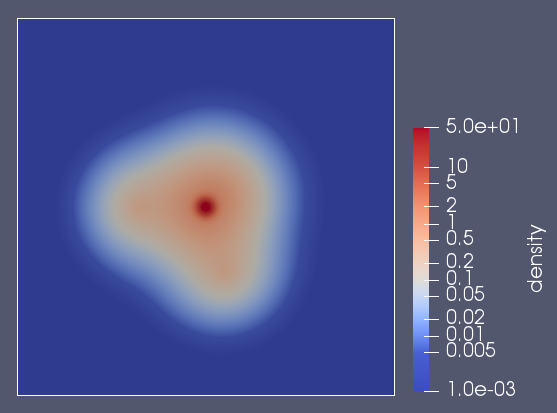
\includegraphics[width=0.48\textwidth]{h2o_density.png}
	\caption{Density plot of the final optimised \ce{H2O}
	Hartree-Fock geometry with a
	\ce{O-H} bond length of \unit[0.95046]{\AA} and
	a \ce{H-O-H} bond angle of $106.35^\circ$.
	A geometry optimisation in ORCA~\cite{ORCA}
	employing the same basis set
	agrees with this result within the convergence tolerance of $10^{-5}$.
	}
	\label{fig:OptimalGeometryWater}
\end{figure}

%%% Local Variables:
%%% mode: latex
%%% TeX-master: "paper"
%%% End:

\section{Current state and future of the program}
\label{sec:state}

\todoil{Maybe refer to the figures in the design section?}

\molsturm currently allows to perform Hartree-Fock calculations
on small molecules using GTO basis functions or using Coulomb-Sturmians.
For the former type of basis functions \gint offers interfaces
to the backend libraries \libint and \libcint and for the latter
type various implementations inside \sturmint are available.
During the SCF procedure \molsturm automatically switches between different
SCF algorithms, currently tODA and a coefficient-based Pulay DIIS,
in order to achieve a good balance between convergence and cost for each iteration.
The default guess are the orbitals resulting from a diagonalisation of the core Hamiltonian,
but the user is free to supply any arbitrary guess from the \python interface.
This includes orbitals from a previous HF calculation or even a totally random guess.
By default \molsturm tries to choose an ARPACK-based eigensolver algorithm
in case the structure of the problem matrix and the other Hartree-Fock
parameters allow this.
What results form this is a fully \contraction-based SCF procedure,
where the Fock matrix is never built in memory at all.
Again the default behaviour can be influenced by the means of suitable
parameters.

After the SCF procedure the quantities like the core Hamiltonian,
the Fock matrix and the electron repulsion integrals
are available via a convenient syntax for post-processing in \python.
This has been demonstrated for example in section \ref{sec:ex:ccd}.
These result objects are also used to realise a simple  MP2 implementation
within \molsturm and to interface to third-party libraries:
Currently MP3 as well as ADC(1), ADC(2)-s, ADC(2)-x and ADC(3)
are available via the \adcman package
and Full-CI can be performed using \pyscf.

Furthermore these HF results can be archived in HDF5 format
in order to restore the full state of the finalised calculation at a later point.
Especially for larger cases where the computations take considerable time,
this allows to perform the SCF on a cluster in advance and
transfer the archived result to a local machine for analysis.
Since the archive contains the full state
including the orbital coefficients and the repulsion integrals,
the local analysis can make use of these quantities
when extracting potential energy surfaces or plotting MOs.
This can be done conveniently in an iteractive \python shell
or a Jupyter notebook for instant feedback.

\molsturm aids with the task of analysing the SCF results
by providing a few basic utility functions.
For example the function values of the SCF orbitals can be exported on an
arbitrary shaped grid to a \numpy array.
This array can than be further manipulated or
plotted in third party libraries or programs.

% What does the molsturm ecosystem consist of right now
%    - python interface to run HF calculations
%        - SCF switches between different algorithms automatically
%    - keywords to select integral backend and control parameters for calculation
%        - sturmint and libint, libcint (multiple backends)
%        - selection of the guess (random, previous, hcore)
%        - selection of the eigensolver
%    - archival of intermediate results and state in HDF5 format
%        - allows to perform big calculation on cluster
%        - restore archive later in a local session
%        - analyse results interactively in a shell or a browser
%    - interactive investigation of results:
%        - summary of SCF
%        - easy access to all relevant quantities (including fock, hcore and eri)
%        - obtain MO data or density on grid for plotting or to 
%    - interface to posthf methods
%        - adcman
%        - pyscf
%    - LA backend:
%        - Bohrium
%        - LAPACK / armadillo
% What is planned for the future
%    - DFT using libxc (gscf has the flexibility)
%    - More analysis tools (direct export of data to standardised output formats like VTK)
%    - Plot wavefunction directly to VTK
%    - openbabel to parse third-party input formats
%    - other standards to interface to further external methods
%    - SCF switching criteria
%    - lazyten
%    - More clever structures for exported quantities

Even though the \python interface of \molsturm allows to control many
aspects of the computation,
there are still a couple of directions for possible improvement.
Most importantly the underlying storage format used
for the Fock matrix or the repulsion integrals are plain and flat \numpy arrays.
In other words the inherent symmetry properties due to spin or index permutations
are entirely unused
giving rise to a much larger memory requirement than theoretically possible.
We currently pay this price in order to make use of the simple and intuitive
syntax employed by \numpy.
For supporting larger problems it is,
however, certainly necessary to replace this by a data structure,
which implicitly considers these symmetries.

One way to do this would be to extend the capabilities of \lazyten.
Right now it only allows to use lazy matrices,
i.e. structures supporting matrix-matrix and matrix-vector
multiplication.
In order to transparently make use of the symmetry and spin structure
of the repulsion integral tensor for example,
we would require lazy tensors,
which support arbitrary \contraction calls.
If we choose the interfaces of such lazy tensors to reflect
the interface of \numpy,
one could get the best of both worlds.
The bohrium project,
which is one of the available computational backends inside \lazyten already,
uses a vary similar approach in their interface,
which we aim at incorporating into our project, too.

Apart from \lazyten there are a couple of other directions,
where molsturm could be easily extended.
This includes making use of the generality of the SCF procedure
in order to support further types of basis functions.
Next steps could be to include basis functions based on
a finite-difference approximated radial function or
further Sturmian basis functions like molecular Sturmians.

Similarly solving the Kohn-Sham equations or the Hartree-Fock
is conceptionally very simple,
since one plainly substitutes the HF exchange term by an appropriate
term representing the exchange-correlation functional.
In the language of lazy matrices one therefore just needs to implement
one extra lazy matrix for representing exchange-correlation functionals
in order to be able to perform density-functional theory
calculations with \molsturm in a basis-function independent way.

Another angle for future work would be to integrate more
closely with the existing \emph{de facto} standards of quantum-chemical software.
On the one hand we plan to use \texttt{openbabel} in order to
support setting up calculations in \molsturm using a range of already existing
input formats.
Similarly we want to integrate routines to export
the orbital coefficients or the denisity to cube or VTK files for plotting
or to export the HF results in MolPro's FCIDUMP or the molden format
for interfacing with other third-party programs.

\section{Take-away}

